\documentclass[11pt,a4paper,english,makeidx]{report}
\usepackage{mathptmx}
\renewcommand{\ttdefault}{mathptmx}
\usepackage[T1]{fontenc}
\usepackage[latin9]{inputenc}
\setcounter{secnumdepth}{3}
\setcounter{tocdepth}{3}
\usepackage{url}
\usepackage{graphicx}
\usepackage{latexsym}
\usepackage{mathptmx}
\usepackage{url}
\usepackage{graphics}
\usepackage{mathptmx}
\renewcommand{\ttdefault}{mathptmx}
\usepackage[T1]{fontenc}
\usepackage[latin9]{inputenc}
\setcounter{secnumdepth}{3}
\setcounter{tocdepth}{3}
\usepackage{url}
\usepackage{graphicx}
\usepackage{babel}

%
%
\makeatletter
\def\maketitle{%
  \null
  \thispagestyle{empty}%
  \vfill
  \begin{center}\leavevmode
    \normalfont
    {\LARGE \@title\par}%
    \vskip 1cm
    {\Large \@author\par}%
    \vskip 1cm
    {\Large \@date\par}%
  \end{center}%
  \vfill
  \null
  \cleardoublepage
  }
\makeatother
\title{User Guide for the Overture Plug-in for Eclipse}
\author{David Holst M\o ller and Christian Thillemann}
\date{2009}



\begin{document}
\maketitle


\section*{Versions:}



\begin{tabular}{|c|c|c|}
\hline 
date & Version & Comment\tabularnewline
\hline
\hline 
03.06.2009 & 0.0.1 & First version of the user guide. Overture
IDE\tabularnewline
\hline
\end{tabular}

% Figures and Tables
\newtheorem{fig}{Figure}\newtheorem{tab}{Table}

% Counter commands
\setcounter{page}{1} \setcounter{chapter}{0} \setcounter{secnumdepth}{4}
\setcounter{tocdepth}{3}

% Page Headings
% Chapter headings are in chapter files
\pagestyle{myheadings}


% TOC
\pagenumbering{roman}
\pagestyle{headings}
\tableofcontents

\pagebreak
% MAIN FILESs 

\pagenumbering{arabic}
\section{Introduction}

The Vienna Development Method (VDM)is one of the longest established
model-oriented formal methods for the development of computer-based
systems and software
\cite{Bjorner&78,Jones90a,Fitzgerald&08c}. It consists of a
group of mathematically well-founded languages for expressing system
models during early design stages, before expensive implementation
commitments are made. The construction and analysis of the model using
Overture help to identify areas of incompleteness or ambiguity in
informal system specifications, and provide some level of confidence
that a valid implementation will have key properties, especially those
of safety or security. VDM has a strong record of industrial
application, in many cases by practitioners who are not specialists in
the underlying formalism or logic
\cite{Larsen&95b,Clement&99,Kurita&09}. Experience with the method
suggests that the effort expended on formal modeling and analysis can
be recovered in reduced rework costs arising from design errors.

VDM models are expressed in a specification language (VDM-SL) that
supports the description of data and functionality
\cite{ISOVDM96a,Fitzgerald&98b,Fitzgerald&09}. Data are defined by
means of types built using constructors that define structured data
and collections such as sets, sequences and mappings from basic values
such as Booleans and numbers. These types are very abstract, allowing
the user to add any relevant constraints as data type
invariants. Functionality is defined in terms of operations over these
data types. Operations can be defined implicitly by preconditions and
postconditions that characterize their behavior, or explicitly by
means of specific algorithms. An extension of VDM-SL, called VDM++,
supports object-oriented structuring of models and permits direct
modeling of concurrency \cite{Fitzgerald&05}. An additional extension
to VDM++ is called VDM Real Time (VDM-RT) (formerly called VDM In a
Constrained Environment (VICE)) \cite{Mukherjee&00,Verhoef&06b}. All
these different dialects are supported by the unified tool called Overture.

Since the VDM modeling languages have a formal mathematical semantics,
a wide range of analyses can be performed on models, both to check
internal consistency and to confirm that models have emergent
properties. Analyses may be performed by inspection, static analysis,
testing or mathematical proof. To assist in this process, Overture
supply tool support for building models in collaboration with other
modeling tools, to execute and test models and to carry out different
forms of static analysis \cite{Larsen&10a}. It can be seen as an open
source version of the commercial tool called VDMTools
\cite{Elmstrom&94,Fitzgerald&08a} although that also have features to
generate executable code in high-level programming languages which are
not yet available in Overture.

This guide explains how to use the Overture IDE for developing models
for different VDM dialects. This user manual starts with explanantion
about how to get hold of the software in
Ssection~\ref{sec:install}. This is followed in
Section~\ref{sec:vdmsupport} with an introduction to the concepts used
in the different Overture perspectives based on Eclipse
terminology. In Section~\ref{sec:projects} it is explained how
projects are managed in the Overture IDE. In Section~\ref{sec:editVDM}
the features supported when editing VDM models are explained. This is
followed in Section~\ref{sec:debug} with an explainantion of the
interpretation and debugging capabilities in the Overture
IDE. Section~\ref{sec:testcoverage} then illustates how test coverage
information can be gathered when models are interpreted. Afterwards
Section~\ref{sec:prettyprint} shows how models with and without test
coverage information can be generated to the text processing system
\LaTeX\ and automatically converted to \texttt{pdf} format if one have
\texttt{pdflatex} installed on the computer. Afterwards from
Section~\ref{sec:POmanagement} to Section~\ref{sec:showlog} different
VDM specfic features are explained. In Section~\ref{sec:POmanagement}
the use of the notion for proof obligations and its support in
Overture is explained. In Section~\ref{sec:testing} a notion of
combinatorial testing and the automation support for that in Overture
is presented. In Section~\ref{sec:vdmuml} support for mapping between
object-oriented VDM models to and from UML models is presented. In
Section~\ref{sec:ToVDMRT} it is illustrated how one can move from a
VDM++ project to a new VDM-RT project. In Section~\ref{sec:showlog} it
is shown how support to analysing and displaying logs from executing
such VDM-RT models. After these sections the main part of the user
manual is completed in Section~\ref{sec:commandline} with an
explanantion of the features from Overture that also is available from
a command-line interface.
Finally in
Appendix~\ref{sec:index} an index of significant terms used in this
user manual can be found. 


\section{Getting Hold of the Software}\label{sec:install}

The Overture project is managed on SourceForge.  The best way to run
Overture is to download a special version of Eclipse with the Overture
functionality already pre-installed. If you go to:
  \begin{quote}
  \url{http://sourceforge.net/projects/overture/files/}
  \end{quote}
  \noindent you can find
  pre-installed versions of Overture for Windows, Linux and Mac. At a
  later stage it will also be possible to use an update site to
  install it from directly in Eclipse. However, at the moment only
  stand-alone versions are distributed because the risk of version
  problems and dependencies with other plug-ins is much smaller this way.

Zip files with a large collection of existing VDM-SL, VDM++ and VDM-RT
projects can be downloaded from
\begin{quote}
\url{http://sourceforge.net/projects/overture/files/Examples/}
\end{quote}
Such existing projects can be imported as described in
subsection~\ref{subsec:importproj}. 

\section{Using the Overture Perspective}\label{sec:vdmsupport}

\subsection{Getting into the Eclipse Terminology}

Eclipse is an open source platform based around a \emph{workbench}\index{workbench} that provides
a common look and feel to a large collection of extension products. Thus if a
user is familiar with one Eclipse product, it will generally be easy to
start using a different product on the same workbench. The Eclipse workbench consists
of several panels known as \emph{views}\index{view}, such as the Script Explorer view at the
top left of Figure~\ref{fig:userguire:OverturePerspective}. A collection of
panels is called a \emph{perspective}\index{perspective}, for example
Figure~\ref{fig:userguire:OverturePerspective} shows the standard Overture
perspective. This consists of a set of views for managing Overture projects and
viewing and editing files in a project. Different perspectives are available in
Overture as will be described later, but for the moment think about a perspective as a
useful composition of views for conducting a particular task.

\begin{figure}[!h]
\begin{center}
  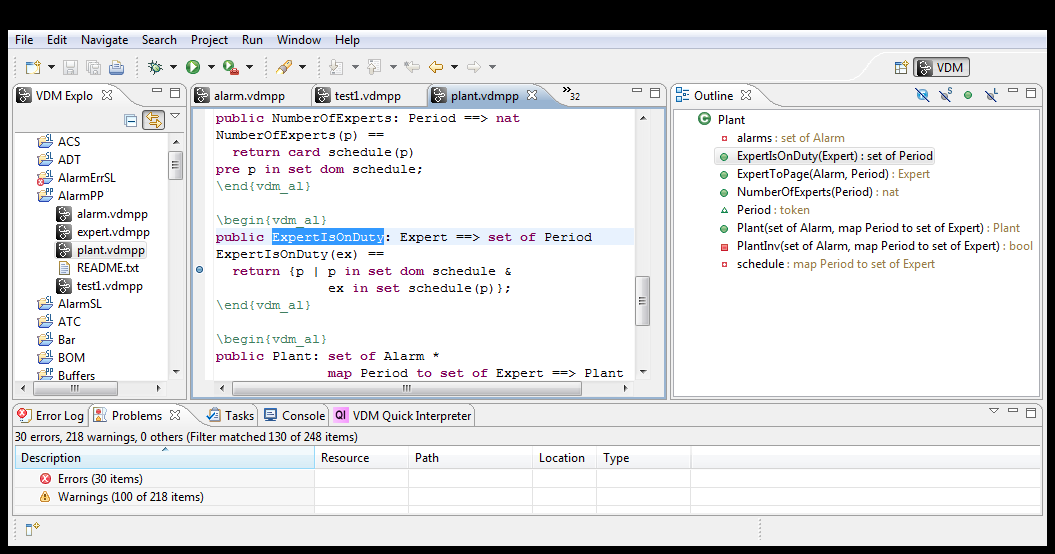
\includegraphics[width=\textwidth]{figures/OverturePerspective}
  \caption[labelInTOC]{The Overture Perspective}
  \label{fig:userguire:OverturePerspective}
\end{center}
\end{figure}

The \emph{Script Explorer view}\index{explorer} lets you create, select, and delete Overture 
projects and navigate between the files in these projects. 

Depending upon the dialect of VDM used in a given project,
a corresponding Overture editor will be available here. A new VDM-SL
project is created choosing the \emph{File} $ \rightarrow$ \emph{New}
$\rightarrow$ \emph{Project}. Then
Figure~\ref{fig:userguide:newOvertureProjectSL} will appear and \emph{Next} can
be used and then a name needs to be given to the project.


\begin{figure}[!h]
\begin{center}
  \caption[labelInTOC]{Creating a New VDM-SL Project}
  \label{fig:userguide:newOvertureProjectSL}
  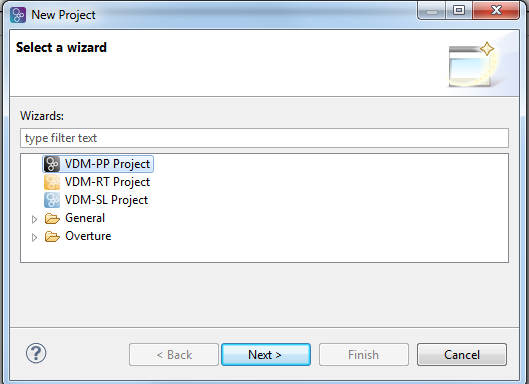
\includegraphics[width=2.5in]{figures/newovertureSLproject}
\end{center}
\end{figure}


The \emph{Outline view}\index{outline}, to the right of the editor (see
Figure~\ref{fig:userguide:OutlineView}), presents an outline of the file selected
in the editor. The outline displays any declared VDM-SL modules, as well as
their state components, values, types, functions and operations. In
case of a flat VDM-SL model the module is called {\ttfamily{DEFAULT}}.\index{DEFAULT}
% and traces.
Figure~\ref{fig:userguire:OverturePerspective} shows the outline view on the
right hand side. Clicking on an operation or function will move the cursor in
the editor to the definition of the operation. At the top of the outline view there
is a button to optionally sort what is
displayed in the outline view, for instance it is possible to hide variables.


\begin{figure}[!h]
\begin{center}
  \caption[labelInTOC]{The Outline View}
  \label{fig:userguide:OutlineView}
  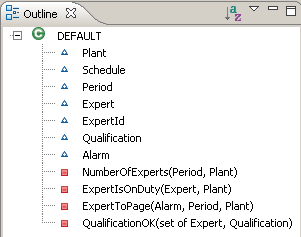
\includegraphics[width=2.5in]{figures/OutlineView}
\end{center}
\end{figure}

The \emph{Problems view}\index{problems} gathers information messages about the projects you are
working on. This includes information generated by Overture, such as
warnings and errors.

Most of the other features of the workbench, such as the menus and
toolbars, are similar to other Eclipse applications, though note that
there is a special menu with Overture specific functionality. One
convenient feature is a toolbar of shortcuts to switch between
different perspectives that appears on the right side of the screen;
these vary dynamically according to context and history.

\subsection{Additional Eclipse Features Applicab�e in Overture}


\section{Managing Overture Projects}\label{sec:projects}

\subsection{Importing Overture Projects}\label{subsec:importproj}


\subsection{Creating a New Overture Project}
\begin{enumerate}
	\item Create a new project by choosing \emph{File}
          $\rightarrow$ \emph{New} $\rightarrow$ \emph{Project}
          $\rightarrow$ \emph{Overture}; 
	\item Select the VDM dialect you wish to use (VDM-SL, VDM-PP
          or VDM-RT);
        \item Type in a project name
	\item Chose whether you would like the contents of the new
          project to be in your workspace or outside from existing
          source files and
        \item click
	the finish button (see \ref{fig:CreateProjectWizard}).
\end{enumerate}

\begin{figure}[!h]
	\begin{center}
	  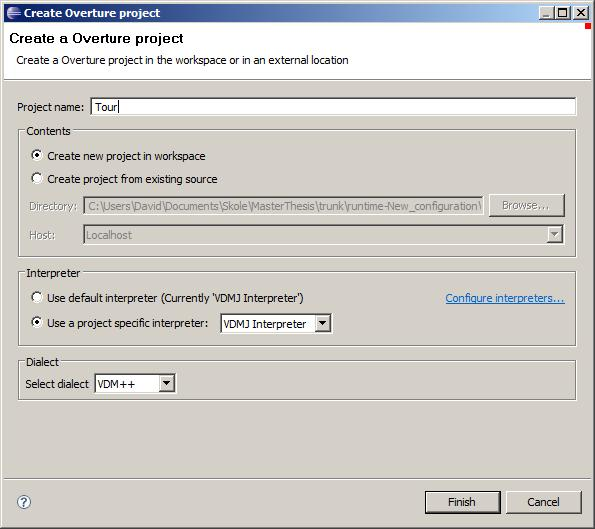
\includegraphics[scale=0.8]{figures/CreateProjectWizard}
	  \caption[Create Project Wizard]{Create Project Wizard}
	  \label{fig:CreateProjectWizard}
	\end{center}
\end{figure}

%%%%%%%%%%%%%%%%%%%%%%%%%%%%%%%%%%
%  Creating a new file
%%%%%%%%%%%%%%%%%%%%%%%%%%%%%%%%%%

\subsection{Creating Files}

Switching to the Overture perspective will change the layout of the user
interface to focus on the VDM development. To change perspective go to the menu 
window $\rightarrow$ open perspective $\rightarrow$ other\ldots and choose the
Overture perspective.
When the developer is in the Overture Perspective the user can create files
using one of the following methods:

\begin{enumerate}
  \item Choose \emph{File} $\rightarrow$ \emph{New} $\rightarrow$
    \emph{VDM-SL Module} or \emph{VDM-PP Class} or \emph{VDM-RT Class} or
  \item Right click on the Overture project where you would like to
    add a new file and then choose \emph{New} $\rightarrow$ $\rightarrow$
    \emph{VDM-SL Module} or \emph{VDM-PP Class} or \emph{VDM-RT Class}.
\end{enumerate}

In both cases one needs to choose a file name and optionally choose a
directory if one does not want to place the file in the directory for
the chosen Overture project. Then a new file with the appropriate file
extension according to the chosen dialect will be created in the
selected directory. This file will use the appropriate module/class
template to get the user started with defining the module/class meant
to be placed in this new file. Naturally keywords for kinds of
definitions that will not be used can be deleted.

\subsection{Setting Project Options}\label{subsec:options}


\section{Editing VDM models}\label{sec:editVDM}


\section{Interpretation and Debugging in Overture}\label{sec:debug}

This section describes how to debug a model using the Overture IDE. 

\subsection{Debug configuration}

Debugging the model under development is done by creating a debug configuration
\index{debug configuration}
from the menu \emph{Run} $\rightarrow $ \emph{Debug configuration}
\ldots 
The debug
configuration dialog requires the following information as input to start the
debugger: the project name, the class, the starting operation/function and the
file containing the starting operation/function.
Figure~\ref{fig:userguide:debugConfiguration} shows a debug configuration,
clicking one of the browse buttons will open a dialog which give the user a list
of choices. The class and operation/function are chosen from the dialog with the
list of expandable classes, if the operation or function have arguments these
must be typed in manually.

\begin{figure}[htp]
\begin{center}
  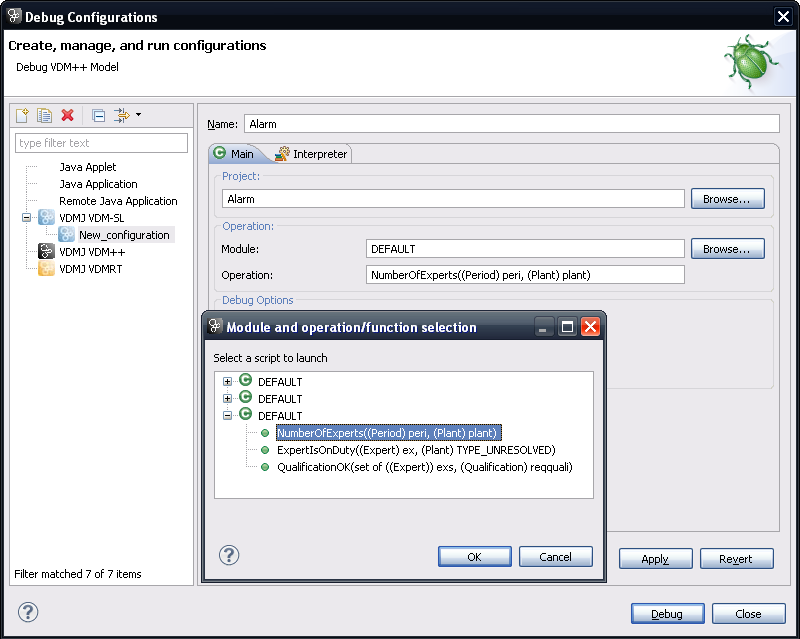
\includegraphics[width=380px]{figures/debugConfiguration}
  \caption{The debug configuration dialog}
  \label{fig:userguide:debugConfiguration}
\end{center}
\end{figure}

\subsection{Debug Perspective}

The Debug Perspective\index{debug perspective} contains the views
needed for debugging in VDM. Breakpoints can easily be set at desired
places in the model, by double clicking in left margin. When the
debugger reaches the location of the breakpoint, the user can inspect
the values of different identifiers and step through the VDM model
line by line.
 
The debug perspective shows the VDM model in an editor as the one used in the
Overture Perspective, but in this perspective there are also views useful during
debugging. The features provided in the debug perspective are described below.
The Debug Perspective is illustrated on figure~\ref{fig:userguide:DebuggingVDM}

\begin{figure}[htp]
\begin{center}
  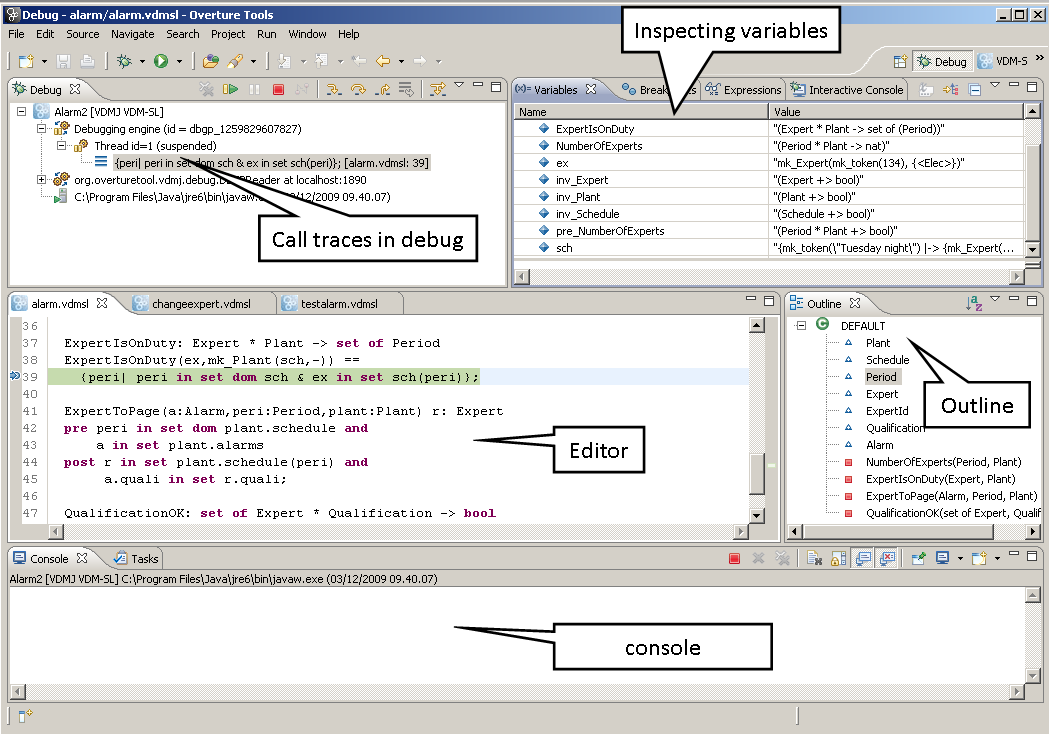
\includegraphics[width=380px]{figures/DebuggingVDM}
  \caption[Debugging perspective]{Debugging perspective}
  \label{fig:userguide:DebuggingVDM}
\end{center}
\end{figure}


\subsubsection{Debug View}

The debug View is located in the upper left corner in the Debug Perspective -
see figure \ref{fig:userguide:DebuggingVDM}. The debug view shows all running
models and the call stack belonging to them. It also displays whether a given model is
stopped, suspended or running. In the top of the view buttons
for debugging such as; stop, step into, step over, resume, etc.\ are located.
All threads are also shown, along with their running status. It is possible to
switch between threads from the Debug View.

\subsubsection{Variables View}
 
This view shows all the variables in a given context, when a breakpoint is
reached. The variables and their values displayed are automatically updated when
stepping through a model. The variables view is by default located in the upper
right hand corner in the Debug Perspective. It is also possible to inspect complex variables,
expanding nested arrays and so forth.

\subsubsection{Breakpoints View}

Breakpoints can be added both from the edit perspective and the debug perspective
from the editor view. In the debug perspective however, there is a breakpoints
view that shows all breakpoints. From the breakpoints view the user can easily
navigate to the location of a given breakpoint, disable, delete or set the hit
count or a break condition. In figure \ref{fig:userguide:DebuggingVDM} the
Breakpoints View is hidden behind the Variables View in the upper right hand 
corner in a tabbed notebook. Section~\ref{sec:userguide:breakpoints} explains
how to use conditional breakpoints.

\subsubsection{Expressions View}

The expressions view allows the user to write expressions, as for the
variables view, the expressions are automatically updated when stepping.
Watch expressions can be added manually or created by selecting 'create watch
expression' from the variables view. It is of course possible to edit existing
expressions. Like the Breakpoints View this view is hidden in the upper right
hand corner.

\subsubsection{Interactive Console View}

While the Expressions View allows to easily inspect values, the functionality is
somewhat limited compared with the functionality provided by VDMTools. For more
thorough inspections the Interactive Console View is more suited. Here commands
can be executed on the given context, i.e.\ where the debugger is at a
breakpoint. The Interactive console keeps a command history, so that already
executed commands can be run again without actually typing in the command all
over. Figure~\ref{fig:userguide:interactiveConsole} shows the interactive
console.

\begin{figure}[htp]
\begin{center}
  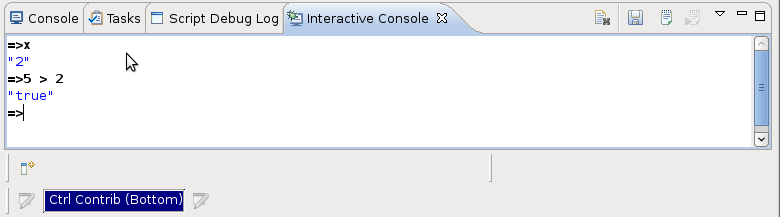
\includegraphics[width=300px]{figures/InteractiveConsole}
  \caption{The interactive console}
  \label{fig:userguide:interactiveConsole}
\end{center}
\end{figure}

\subsubsection{Conditional breakpoints}
\label{sec:userguide:breakpoints}

Conditional breakpoints can also be defined. These are a powerful tool for the
developer since it allows specifying a condition for one or more variables which
has to be true in order for the debugger to stop at the given breakpoint. Apart
from specifying a break condition depending on variables, a hit count can also be
defined. A conditional breakpoint with a hit count lets the user specify a given
number of calls to a particular place at which the debugger should break.

Making a breakpoint conditional is done by right clicking on the breakpoint
mark in the left margin and select the option Breakpoint properties\ldots This
opens a dialog like the one shown in
figure~\ref{fig:userguide:BreakpointConditional}. It is possible to choose
between two different conditional breakpoints, a hit count condition and one
based on an expression defined by the user. 

\begin{figure}[htp]
\begin{center}
  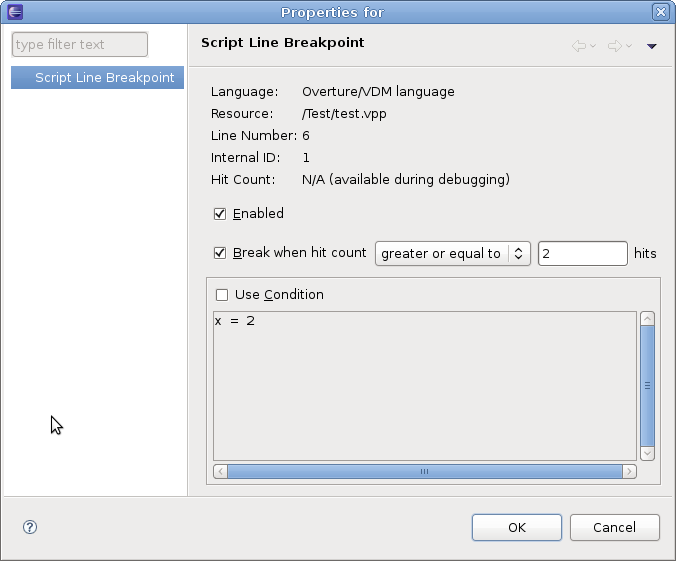
\includegraphics[width=250px]{figures/Breakpointconditional}
  \caption{Conditional breakpoint options}
  \label{fig:userguide:BreakpointConditional}
\end{center}
\end{figure}

\section{Collecting Test Coverage Information}\label{sec:testcoverage}


\section{Pretty Printing to \LaTeX}\label{sec:prettyprint}

\section{Managing Proof Obligations}\label{sec:POmanagement}


\section{Combinatorial Testing}\label{sec:testing}

%A specific manual for this topic exist, please refer to \cite{CTManual}.

\section{Mapping VDM++ back and forth to UML}\label{sec:vdmuml}

\section{Moving from VDM++ to VDM-RT}\label{sec:ToVDMRT}

\section{Analysing and Displaying Logs from VDM-RT Executions}\label{sec:showlog}

\section{A Command-Line Interface to VDMJ}\label{sec:commandline}



\end{document}